\documentclass[12pt, a4paper]{article}
\usepackage{amsthm}
\usepackage{amsmath}
\usepackage{amssymb}
\usepackage{amsfonts}
\usepackage{algorithm}
\usepackage{algpseudocode}
\usepackage{graphicx}
\usepackage{verbatim}
\usepackage{hyperref}
\usepackage{listings}
\usepackage{xcolor}
\usepackage{url}
\usepackage[utf8]{inputenc}
\usepackage[english,russian]{babel}
\usepackage{tabularx}
\usepackage{subcaption}
\usepackage{geometry}
\usepackage{booktabs}
\usepackage{caption}

\definecolor{codegreen}{rgb}{0,0.6,0}
\definecolor{codegray}{rgb}{0.5,0.5,0.5}
\definecolor{codepurple}{rgb}{0.58,0,0.82}
\definecolor{backcolour}{rgb}{0.95,0.95,0.92}

\lstdefinestyle{mystyle}{
  commentstyle=\color{codegreen},
  keywordstyle=\color{magenta},
  numberstyle=\tiny\color{codegray},
  stringstyle=\color{codepurple},
  basicstyle=\ttfamily\footnotesize,
  breakatwhitespace=false,
  breaklines=true,
  captionpos=b,
  keepspaces=true,
  numbers=left,
  numbersep=5pt,
  showspaces=false,
  showstringspaces=false,
  showtabs=false,
  tabsize=2,
  columns=fullflexible
}

\lstdefinelanguage{yaml}{
  keywords={true,false,null,yes,no},
  keywordstyle=\color{magenta},
  comment=[l]{\#},
  commentstyle=\color{codegreen},
  stringstyle=\color{codepurple},
  morestring=[b]',
  morestring=[b]",
  sensitive=false,
}

\lstset{style=mystyle}
\lstset{basicstyle=\ttfamily}
\AddToHook{env/lstlisting/begin}{\lstset{basicstyle=\ttfamily\normalsize}}

\title{Агентное моделирование экономических систем на основе больших языковых моделей}
\author{Матвей Назаров}

\begin{document}

\thispagestyle{empty}

\begin{center}
% ФЕДЕРАЛЬНОЕ ГОСУДАРСТВЕННОЕ БЮДЖЕТНОЕ\\
% ОБРАЗОВАТЕЛЬНОЕ УЧРЕЖДЕНИЕ ВЫСШЕГО ОБРАЗОВАНИЯ\\
САНКТ-ПЕТЕРБУРГСКИЙ ГОСУДАРСТВЕННЫЙ УНИВЕРСИТЕТ\\
% (СПбГУ)\\
\vspace{1.5cm}
\textbf{\large Назаров Матвей Антонович} \\
\vspace{0.7cm}
\textbf{\large Выпускная квалификационная работа}\\
\vspace{0.7cm}
\textbf{\large Агентное моделирование экономических систем на основе больших языковых моделей}
% Образовательная программа бакалавриата <<Науки о данных>>
\vfil\vfil
Уровень образования: бакалавриат

Направление 02.03.01 <<Математика и компьютерные науки>>

Образовательная программа CB.5189.2022 <<Науки о данных>>
% \includegraphics[width=0.35\textwidth]{images/spbu_logo}
% \vfil\vfil
% \textbf{\large Дипломная работа}\\
% \textbf{\large <<Об обратимых структурах данных>>}
\end{center}

% \begin{center}
% ФЕДЕРАЛЬНОЕ ГОСУДАРСТВЕННОЕ БЮДЖЕТНОЕ\\
% ОБРАЗОВАТЕЛЬНОЕ УЧРЕЖДЕНИЕ ВЫСШЕГО ОБРАЗОВАНИЯ\\
% ``САНКТ-ПЕТЕРБУРГСКИЙ ГОСУДАРСТВЕННЫЙ УНИВЕРСИТЕТ''\\
% (СПбГУ)\\
% \vfil
% Образовательная программа бакалавриата <<Науки о данных>>
% \vfil\vfil
% \includegraphics[width=0.35\textwidth]{images/spbu_logo}
% \vfil\vfil
% \textbf{\large Дипломная работа}\\
% \textbf{\large <<Агентное моделирование экономических систем на основе больших языковых моделей>>}
% \end{center}

\vfil\vfil
\noindent\hfill
\begin{minipage}{0.6\textwidth}
\raggedleft
Научный руководитель:\\
Николаев Максим Сергеевич\\
Научный сотрудник, Лаборатория искусственного интеллекта, математики и компьютерных наук им.~А.\,А.~Маркова

\bigskip
Рецензент:\\
Максудова Зарина Маратовна,\\
Аналитик-разработчик, ООО <<Яндекс>>
\end{minipage}

\vfil\vfil
\begin{center}
Санкт-Петербург\\
2026
\end{center}
\eject

\tableofcontents
\newpage

\sloppy

\section{Введение}

Эта работа про то, можно ли заставить языковую модель играть роль экономических агентов так, чтобы результат был не просто похожим на реальность, а количественно проверяемым. Конкретный вопрос звучит так: если запустить несколько десятков агентов, каждый из которых принимает решения через LLM на основе своей биографии и текущей рыночной ситуации, воспроизведут ли они классические стилизованные факты макроэкономики - кривую Оукена, кривую Беверидж, кривую Филлипса, импульсные отклики на шоки? И если да - можно ли подобрать параметры так, чтобы симулированные статистики были близки к реальным данным ФРС?

Агентные модели существуют в экономике уже больше тридцати лет. Они хорошо работают для сложных нелинейных систем, но у них есть старая проблема: поведенческие правила агентов приходится задавать руками, и эти правила произвольны. Большие языковые модели предлагают выход: если модель обучена на текстах о человеческом поведении, она может сама <<вывести>> подходящее решение из контекста, не требуя жёсткого кодирования.

Главный методологический вклад работы~- это не сама идея LLM-ABM (её уже делали другие), а строгая количественная валидация. Параметры модели откалиброваны к девяти моментам реальных данных FRED (безработица, инфляция, выпуск, Оукен, Беверидж, Филлипс) методом симулированных моментов; построены bootstrap доверительные интервалы для импульсных откликов. Ни EconAgent, ни SimCity~- ближайшие аналоги в литературе~- этого не делали.

\section{Обзор предметной области}

\subsection{Агентные вычислительные модели в макроэкономике}

ABM в экономике~- это не какая-то экзотика. Первые серьёзные результаты появились ещё в 1990-х. Люкс и Марчези \cite{lux1999} показали, что простая модель финансового рынка с гетерогенными агентами воспроизводит толстые хвосты распределения доходности~- то, с чем стандартная DSGE-теория вообще не справляется. Потом Дози, Фаджьоло и Ровентини \cite{dosi2010} построили многосекторный ABM с эндогенными инновациями и воспроизвели стилизованные факты бизнес-цикла вообще без прямой калибровки под исторические данные.

Проблема одна и давно известна. Поведенческие правила задаются произвольно. Фаджьоло и Ровентини \cite{fagiolo2017} в своём обзоре написали об этом прямо: <<Основная методологическая слабость ABM состоит в том, что исследователь обладает слишком большой свободой в задании поведенческих правил>>. Никакого хорошего решения до появления LLM не было.

\subsection{LLM как экономические агенты}

Хортон \cite{horton2023} обратил внимание на важную вещь: языковая модель, обученная на огромных объёмах текстов о людях, по сути становится своего рода <<цифровой копией>> человеческого поведения~- он назвал это <<Homo Silicus>>. Если спросить её, как бы человек поступил в той или иной экономической ситуации, она отвечает на основе того, что <<видела>> в текстах: как реальные люди принимали решения в похожих обстоятельствах. Хортон запустил GPT-4 в стандартных поведенческих экспериментах~- игра ультиматума, диктатор, предложение труда~- и показал, что LLM качественно правильно воспроизводит человеческое поведение.

Манниг, Хортон и Ламонт \cite{manning2024} пошли дальше: на выборке из 500 экономических воздействий (например, изменение цен, стимулы к труду и т.п.), измеренных как на реальных людях, так и на LLM-агентах, корреляция получилась $r = 0.85$. Это очень высокий показатель.

Агер и коллеги \cite{aher2023} показали, что при точном задании демографических характеристик LLM воспроизводит распределения ответов реальных людей в психологических экспериментах. Именно этот результат вдохновил подход к биографиям: вместо абстрактных <<типов>> описываются жизненные обстоятельства агентов, из которых тип поведения следует сам собой.

\subsection{LLM-ABM в макроэкономике: что уже сделали}

EconAgent \cite{li2023} (Ли и коллеги, 2023, ACL 2024)~- первая полноценная LLM-ABM с рынком труда и рынком товаров. Авторы показывают, что LLM-агенты воспроизводят более реалистичную безработицу и инфляцию по сравнению с поведенческими ABM. Нет центрального банка, нет прогрессивного налогообложения, нет формальных IRF-тестов и количественной калибровки к реальным данным.

SimCity \cite{feng2025} (Фэн и коллеги, 2025)~- самый масштабный из известных вариантов. Тысяча домохозяйств, 44 категории товаров, 180 шагов симуляции, GPT-4o-mini и GPT-5 для проверки. Авторы качественно показывают, что SimCity воспроизводит кривую Филлипса, закон Оукена, кривую Беверидж. Но в статье прямо написано: модель <<not quantitatively calibrated with real-world data>>.

Моя работа добавляет две вещи, которых нет ни у EconAgent, ни у SimCity: MSM-калибровка к FRED и bootstrap доверительные интервалы для IRF.


\section{Архитектура модели}

\subsection{Общая структура}

Модель~- замкнутая экономика с четырьмя типами агентов. Десять домохозяйств предлагают труд, потребляют товары, платят налоги и получают трансферы и проценты на сбережения. Три фирмы нанимают труд, производят товары и устанавливают цены. Центральный банк проводит денежно-кредитную политику по правилу Тейлора. Правительство собирает прогрессивный налог и равномерно перераспределяет его обратно.

Симуляция идёт дискретными тиками. Никакой жёсткой временной интерпретации нет~- тик может быть неделей, месяцем или кварталом в зависимости от того, что сравнивается с реальными данными.

Порядок действий в каждом тике: сначала центральный банк вычисляет ставку по правилу Тейлора на основе состояния предыдущего периода. Потом все домохозяйства и фирмы параллельно отправляют запросы в языковую модель и получают решения. Затем рынок труда обрабатывается через функцию согласования Мортенсена-Писсаридеса. После этого рынок товаров очищается в выбранном режиме. Правительство собирает налоги и выплачивает трансферы. В конце сохраняются все агрегатные показатели: выпуск, потребление, безработица, инфляция, ставка и реальная зарплата.

Начальные условия для всех прогонов: средняя цена $= 15.0$, средняя зарплата $= 15.0$, начальные деньги каждого домохозяйства $= 200.0$, начальный капитал каждой фирмы $= 1000.0$.

\subsection{Принятие решений агентами}

Ключевое архитектурное решение~- никаких жёстко закодированных поведенческих правил. Агент получает промпт и формулирует решение сам.

В начале каждого периода домохозяйство получает промпт из двух частей. Системный промпт содержит биографию агента. Пользовательский промпт рендерится через Jinja2-шаблон \texttt{household.j2} и содержит текущую рыночную ситуацию: среднюю цену, среднюю зарплату, безработицу, процентную ставку, инфляцию и реальную зарплату, текущее финансовое положение и историю последних 10 периодов.

Ответ языковой модели парсится в структуру \texttt{HouseholdDecision} с четырьмя полями: текст рассуждения (\texttt{reasoning}), предложение труда от нуля до единицы (\texttt{labor\_supply}), бюджет на потребление (\texttt{consumption\_budget}) и сумма сбережений (\texttt{savings\_amount}).

Парсер обрабатывает типичные артефакты LLM: римские цифры, словесные описания вроде <<approximately 0.8>>, вложенные JSON, словари вида \texttt{\{"value": 10.5\}}. После парсинга проверяется, что \texttt{labor\_supply} находится в $[0, 1]$, остальные поля не могут быть отрицательными. Благодаря этому симуляция никогда не падает из-за некорректного ответа LLM.

Для фирмы аналогичная структура~- \texttt{FirmDecision}~- содержит рассуждение, спрос на труд (\texttt{labor\_demand}), целевую цену (\texttt{price\_setting}) и целевой объём производства (\texttt{production\_target}).

Температура генерации LLM установлена в $0.7$. Это баланс между детерминированностью и избыточным шумом.

\subsection{Принцип биографий}

Биографии~- отдельная архитектурная идея. Намеренно избегаются <<инструктивные>> биографии вида <<ты сберегательный агент, откладывай 50\% дохода>>. Вместо этого описываются жизненные обстоятельства: кто человек, как он относится к деньгам и почему.

Наташа, 61 год, бухгалтер, которая три года назад овдовела и обнаружила, что муж оставил меньше накоплений, чем они оба предполагали. Она планирует выйти на пенсию через два года. Последнее предложение её биографии: <<Comfort matters far less to you than the feeling that you are not going to run out.>>

Это контекст, а не правило. Языковая модель сама делает вывод, как такой человек должен вести себя с деньгами. Принципиальная разница: если изменится рыночная ситуация, агент адаптирует поведение, потому что он <<понимает>>, почему ведёт себя так, а не выполняет зашитый алгоритм.

Полный список из 10 биографий охватывает широкий профессиональный срез (см.\ Приложение А). Три фирмы: ценовой конкурент с тонкой маржой, качественный производитель с репутацией и молодая агрессивная компания в фазе роста.

\subsection{Рынок труда по модели Мортенсена-Писсаридеса}

Первый вариант модели использовал Бернуллиевское участие: каждое домохозяйство работает с вероятностью, равной его \texttt{labor\_supply}. Это плохо по двум причинам. При малом числе агентов биномиальный шум огромный и маскирует реакцию на рыночные сигналы. Плюс такая схема в принципе не может породить одновременно положительные безработицу и вакансии~- а это необходимое условие для нетривиальной кривой Беверидж.

Поэтому используется функция согласования Кобба-Дугласа стандартного типа Мортенсена-Писсаридеса \cite{mortensen1994}:
\begin{equation}
H = A \cdot U^{\alpha} \cdot V^{1-\alpha},
\end{equation}
где $H$~- число успешных сопоставлений рабочих и вакансий, $U$~- совокупное предложение труда (сумма \texttt{labor\_supply} всех домохозяйств), $V$~- совокупный спрос на труд (сумма \texttt{labor\_demand} всех фирм), $\alpha = 0.5$~- симметричная эластичность, $A$~- эффективность согласования, подбираемая методом моментов.

После вычисления $H$ возникают <<несогласованные>> остатки: $u_{\text{unmet}} = U - H$ незанятых работников и $v_{\text{unfilled}} = V - H$ незаполненных вакансий. При $A < 1$ оба значения положительны одновременно~- это и даёт кривую Беверидж. При $A = 1$ формула упрощается до $H = \min(U, V)$~- бесфрикционный случай.

Рационирование внутри мэтчей пропорциональное: фирма $i$ получает $\text{hired}_i = \text{labor\_demand}_i \cdot (H / V)$, домохозяйство $j$ получает $\text{worked}_j = \text{labor\_supply}_j \cdot (H / U)$.

Ставка разделения $s$ определяет долю прошлых мэтчей, которая возвращается в пул соискателей в начале каждого периода. Это создаёт постоянный приток в безработицу независимо от текущих решений и усиливает персистентность. $s$ тоже калибруется.

Зарплата адаптируется по правилу:
\begin{equation}
w_{t+1} = w_t \cdot \left(1 + \varphi \cdot \frac{V - U}{U}\right),
\end{equation}
где $\varphi = 0.15$. Рост ограничен $+10\%$, снижение - $-5\%$ за период. Уровень безработицы нормируется на рабочую силу: $\text{unemployment\_rate} = u_{\text{unmet}} / U$.

\subsection{Рынок товаров}

Три режима, настраиваемые через параметр \texttt{goods\_clearing\_mode} в YAML-конфиге.

\textbf{Режим average}: все фирмы торгуют по единой средней цене. Выручка распределяется пропорционально долям запасов. Приближение к вальрасианскому равновесию.

\textbf{Режим queue}: покупатели посещают фирмы в порядке возрастания цены~- сначала к самой дешёвой. Каждая фирма торгует по своей цене. Это создаёт дисперсию цен и стратегическое ценообразование.

\textbf{Режим weighted}: спрос направляется к фирмам обратно пропорционально цене~- мягкий вариант без жёсткой очереди.

Для hero IRF прогонов выбран режим queue на основании того, что он единственный даёт правильный знак инфляции при demand shock (см.\ раздел~\ref{sec:modes}).

\subsection{Ценовая коррекция}

Цена фирмы на каждом шаге корректируется частично по схеме Калво:
\begin{equation}
p_t = p_{t-1} + \text{price\_adj} \cdot (p^{\text{LLM}}_t - p_{t-1}).
\end{equation}
При $\text{price\_adj} = 1.0$ цена мгновенно следует за решением LLM. При $\text{price\_adj} < 1.0$~- цена липкая (sticky prices). Параметр \texttt{price\_adj} входит в калибруемый вектор: MSM определил оптимальное значение $0.164$, что соответствует сильной ценовой инерции.

\subsection{Денежно-кредитная политика и налоги}

Центральный банк следует правилу Тейлора \cite{taylor1993}:
\begin{equation}
r_t = \max\!\left(0,\; \min\!\left(0.25,\; r^* + \varphi_{\pi}(\pi_t - \pi^*) + \varphi_u(u^* - u_t)\right)\right).
\end{equation}
Нейтральная ставка $r^* = 0.05$. Цель по инфляции $\pi^* = 0.02$. Цель по безработице $u^* = 0.05$. Параметры $\varphi_{\pi}$ и $\varphi_u$ входят в калибруемый вектор $\theta$.

Когда безработица выше цели, $(u^* - u_t) < 0$, и ставка снижается. Это корректное поведение центрального банка~- стимулировать при росте безработицы. Ограничение ZLB обеспечено через $\max(0, \ldots)$.

Начисление процентов: $\text{savings}_{t+1} = \text{savings}_t \cdot (1 + r_t)$.

Прогрессивный налог в трёх скобках: доход до 20 единиц облагается по ставке 10\%, от 20 до 50~- по 20\%, свыше 50~- по 35\%. Весь собранный налог перераспределяется поровну всем домохозяйствам как трансфер в том же периоде.

\subsection{Память агентов}

Каждый агент ведёт скользящее окно из 10 последних периодов. В окне хранится: номер шага, сколько проработал, сколько заработал, сколько потратил и сколько купил по факту, сколько отдал налогов и получил трансферов, сколько денег осталось. Также в историю попадают рыночные условия того периода.

Выбор окна в 10 периодов~- на меньшем агенты плохо адаптируются к изменениям, на большем~- стоимость API-запросов существенно растёт, а качество решений уже не улучшается при горизонте симуляции в 60 шагов.

Также реализованы периодические рефлексии: каждые \texttt{reflection\_every} шагов агент получает запрос <<подведи итоги прошедшего периода>>.

\subsection{Параллелизм}

Все 13 вызовов языковой модели (10 домохозяйств + 3 фирмы) выполняются через \texttt{asyncio.gather()}~- параллельно в рамках одного тика. Семафор \texttt{max\_concurrency} = 30 предотвращает перегрузку API. Средняя задержка на тик~- 8--15 секунд, определяется самым медленным агентом в батче. Без параллелизма один тик занимал бы 2--3 минуты.

\section{Технический стек и структура кода}

\subsection{Технологии}

Язык~- Python 3.11. Языковая модель~- DeepSeek-V3 (\texttt{deepseek-chat-v3-0324}) через deepseek-api. DeepSeek-V3~- смесь экспертов с 671 млрд параметрами, производительностью сопоставимой с GPT-4o, но значительно дешевле: \$0.27/M входных и \$1.10/M выходных токенов.

Стоимость вычислений принципиально ограничивала масштаб работы. Одна симуляция из 60 тиков с 13 агентами требует порядка 800 вызовов API; при среднем промпте $\approx$1\,200 входных и 300 выходных токенов это составляет около \textbf{\$0.50 за симуляцию}. MSM-калибровка из 41 такой симуляции обошлась примерно в \textbf{\$20}. Hero IRF прогоны~- 15 симуляций по 33 агента на 60 тиков~- ещё \textbf{\$20}. Суммарные расходы на API за всё время разработки~- с учётом отладки, промежуточных прогонов и экспериментов~- составили порядка \textbf{\$60}. Именно ограниченность бюджета объясняет малый размер модели ($N = 13$ агентов для MSM, $N = 30$ для hero прогонов), небольшой горизонт (60 тиков) и всего 5 прогонов на каждый сценарий~- что напрямую сказывается на ширине доверительных интервалов.

Для асинхронных вызовов~- \texttt{asyncio} и \texttt{httpx}. Структурированный вывод~- Pydantic v2: LLM получает JSON Schema из Pydantic-модели и должна вернуть валидный JSON. Шаблоны промптов~- Jinja2. Для численного анализа~- numpy и scipy. Для работы с данными~- pandas. Для графиков~- matplotlib с Agg backend (без GUI). Конфигурация экспериментов~- YAML. Байесовская оптимизация написана на чистом numpy.

\subsection{Структура директорий}

Исходный код лежит в \texttt{src/}. Внутри:
\begin{itemize}
  \item \texttt{src/agents/}~- классы \texttt{HouseholdAgent} и \texttt{FirmAgent};
  \item \texttt{src/llm/}~- клиент API и менеджер промптов;
  \item \texttt{src/core/}~- движок симуляции и логгер;
  \item \texttt{src/economics/}~- реализация рынков;
  \item \texttt{src/schemas/}~- Pydantic-схемы решений;
  \item \texttt{src/analysis/}~- модули MSM, DSGE-baselines и сравнительного анализа.
\end{itemize}

Скрипты запуска~- в \texttt{scripts/}. Конфигурации экспериментов~- в \texttt{config/experiments/}. Результаты (CSV прогонов, JSONL MSM, JSON состояния калибровки)~- в \texttt{data/}. Графики~- в \texttt{charts/v2/}.

\subsection{Конфигурация через YAML}

Каждый эксперимент описывается отдельным YAML-файлом. Там задаётся число агентов, режим рынка товаров, параметры рынка труда, настройки центрального банка, налоговые скобки и события (шоки). Пример структуры события:

\begin{lstlisting}[language=yaml]
events:
  - step: 10
    type: cash_injection
    target: household
    amount: 100.0
    description: "Helicopter Money Drop -- demand shock"
\end{lstlisting}

При запуске движок обрабатывает события в нужный шаг, начисляет деньги агентам и рассылает им уведомления о произошедшем. Параметры из YAML инициализируют объект \texttt{SimulationEngine}. Если нужно перекрыть параметры калиброванным $\theta^*$ из \texttt{state.json}, скрипт \texttt{run\_hero\_irf.py} пробрасывает патч поверх базового конфига.

\subsection{Логирование и воспроизводимость}

Каждый прогон пишет CSV с агрегатными показателями всех периодов. Кроме того, движок пишет JSONL с детальными решениями агентов~- reasoning и все числовые поля.

Seed генератора случайных чисел фиксируется для bootstrap, но не влияет на вывод LLM~- он стохастичен по природе. Поэтому <<воспроизводимость>>~- это воспроизводимость средних статистик по нескольким прогонам, а не отдельного прогона.

\subsection{Тесты}

Двадцать один юнит-тест покрывает критические компоненты: 7 тестов для функции согласования Мортенсена-Писсаридеса, 6 для очистки товарного рынка в трёх режимах, 3 для правила Тейлора, 5 для парсинга Pydantic-ответов. Все 21 тест зелёные.

\section{MSM-калибровка к данным FRED}

\subsection{Зачем вообще калибровать}

Без калибровки модель работает с произвольными параметрами. Например, если параметр эффективности трудоустройства $A$ низкий~- безработица в симуляции будет 40--50\%, что принципиально расходится с реальными 5--6\%. Метод симулированных моментов (MSM)~- стандартный эконометрический инструмент для калибровки структурных моделей. Идея: запустить симуляцию, вычислить моменты (средние, автокорреляции, корреляции) и минимизировать расстояние между симулированными моментами и аналогичными моментами реальных данных.

\subsection{Параметры и цели}

Калибруются пять параметров:
\begin{itemize}
  \item $\varphi_{\pi} \in [0.5,\, 2.5]$~- чувствительность правила Тейлора к инфляции;
  \item $\varphi_u \in [0.0,\, 1.2]$~- чувствительность к безработице;
  \item $A \in [0.35,\, 1.0]$~- эффективность трудоустройства;
  \item $\text{price\_adj} \in [0.10,\, 1.0]$~- скорость Калво-коррекции цен;
  \item $s \in [0.0,\, 0.15]$~- ставка разделения на рынке труда.
\end{itemize}

Целевые моменты вычислены из данных FRED за январь 1990~- декабрь 2024 через fredapi. Используются девять моментов: $\overline{\text{UNRATE}} = 5.67\%$, AR(1) UNRATE $= 0.864$, $\overline{\pi}_{\text{CPI}} = 0.657\%$, std$(\pi) = 0.538\%$, AR(1)$(\pi) = 0.408$, AR(1) $\ln\text{GDP} = 0.999$, корреляция Оукена $= -0.860$, корреляция Филлипса $= -0.241$, корреляция Беверидж $= -0.616$.

Функция потерь~- взвешенная сумма квадратов нормализованных отклонений:
\begin{equation}
J(\theta) = \sum_k w_k \cdot \left(\frac{m^{\text{sim}}_k(\theta) - m^{\text{FRED}}_k}{\sigma_k}\right)^2.
\end{equation}
Веса повышены для <<нагрузочных>> моментов: корреляция Оукена, среднее безработицы, std инфляции.

\subsection{Протокол оптимизации}

Оптимизация шла в три этапа.

\textbf{Первый~- Latin Hypercube Sampling (LHS).} Сформировано 10 точек в 5-мерном пространстве с seed $= 42$, затем ещё 16 точек с seed $= 43$. LHS обеспечивает равномерное покрытие по каждой оси. Для каждой точки запускалась симуляция с 30 домохозяйствами и 60 тиками.

\textbf{Второй~- байесовская оптимизация.} 5 итераций Gaussian Process~- Expected Improvement. Гауссовский процесс с ядром Matern(2.5) обучается на $\log(J+1)$~- логарифм сглаживает огромный диапазон значений $J$. На каждой итерации из 2000 случайных кандидатов выбирается точка с максимальным Expected Improvement.

\textbf{Третий~- perturbation.} Вокруг наиболее перспективных точек 10 прогонов со случайными возмущениями $\pm 20\%$.

Итого 41 вычисление функции потерь.

\begin{figure}[h]
\centering
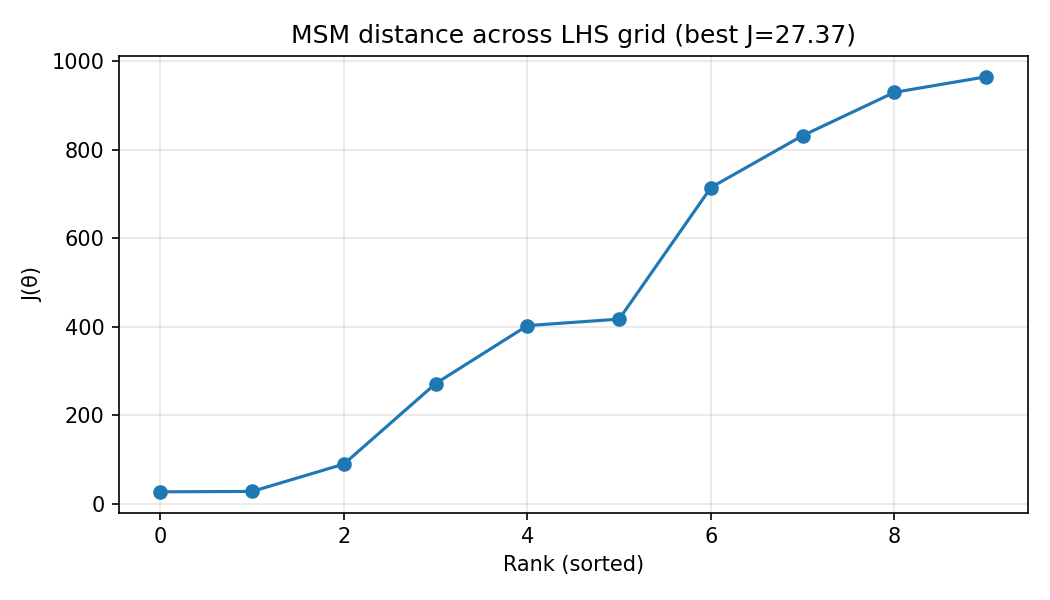
\includegraphics[width=0.75\textwidth]{images/fig_msm_J}
\caption{Ландшафт функции потерь MSM по 41 точке оптимизации. По горизонтали~- порядковый номер вычисления (LHS, байесовская оптимизация, perturbation); по вертикали~- $\log(J+1)$. Видно резкое снижение в процессе поиска.}
\label{fig:msm_J}
\end{figure}

\subsection{Результаты}

Лучшая точка~- lhs2\_004 с $J = 21.79$. Калиброванный вектор $\theta^*$:
\[
\varphi_{\pi} = 1.341,\quad \varphi_u = 0.440,\quad A = 0.977,\quad \text{price\_adj} = 0.164,\quad s = 0.116.
\]

Значение $\varphi_{\pi} \approx 1.34$ близко к классическому правилу Тейлора ($\varphi_{\pi} = 1.5$ в исходной статье Тейлора 1993 года). Это косвенный признак правдоподобности: MSM сам нашёл значение, близкое к теоретически обоснованному.

Значение $A \approx 0.98$ соответствует высокой эффективности согласования. Стандартная калибровка для США по литературе Мортенсена-Писсаридеса даёт $A \approx 0.9$--$1.0$. MSM нашёл то же из данных, без подсказки.

\begin{table}[h]
\centering
\caption{Сравнение симулированных моментов при $\theta^*$ с целевыми моментами FRED.}
\label{tab:moments}
\begin{tabular}{lccc}
\toprule
\textbf{Момент} & \textbf{FRED} & \textbf{Симуляция} & \textbf{Вклад в $J$} \\
\midrule
$\overline{\text{UNRATE}}$ (\%) & 5.67 & 8.72 & 1.55 \\
AR(1) безработицы & 0.864 & 0.866 & $\approx 0$ \\
std инфляции (\%) & 0.538 & 0.257 & 0.12 \\
AR(1) инфляции & 0.408 & 0.976 & 8.06 \\
AR(1) выпуска & 0.999 & 0.913 & 1.47 \\
Корр.\ Оукена & $-0.860$ & $+0.085$ & 9.94 \\
Корр.\ Филлипса & $-0.241$ & $-0.024$ & 0.52 \\
Корр.\ Беверидж & $-0.616$ & $-0.528$ & 0.13 \\
\bottomrule
\end{tabular}
\end{table}

RMSE против FRED: $0.377$. Доля моментов с правильным знаком: $7/9 = 77.8\%$. Некалиброванный baseline даёт $J > 800$. Калибровка сократила дистанцию до FRED примерно в 30--40 раз.

\begin{figure}[h]
\centering
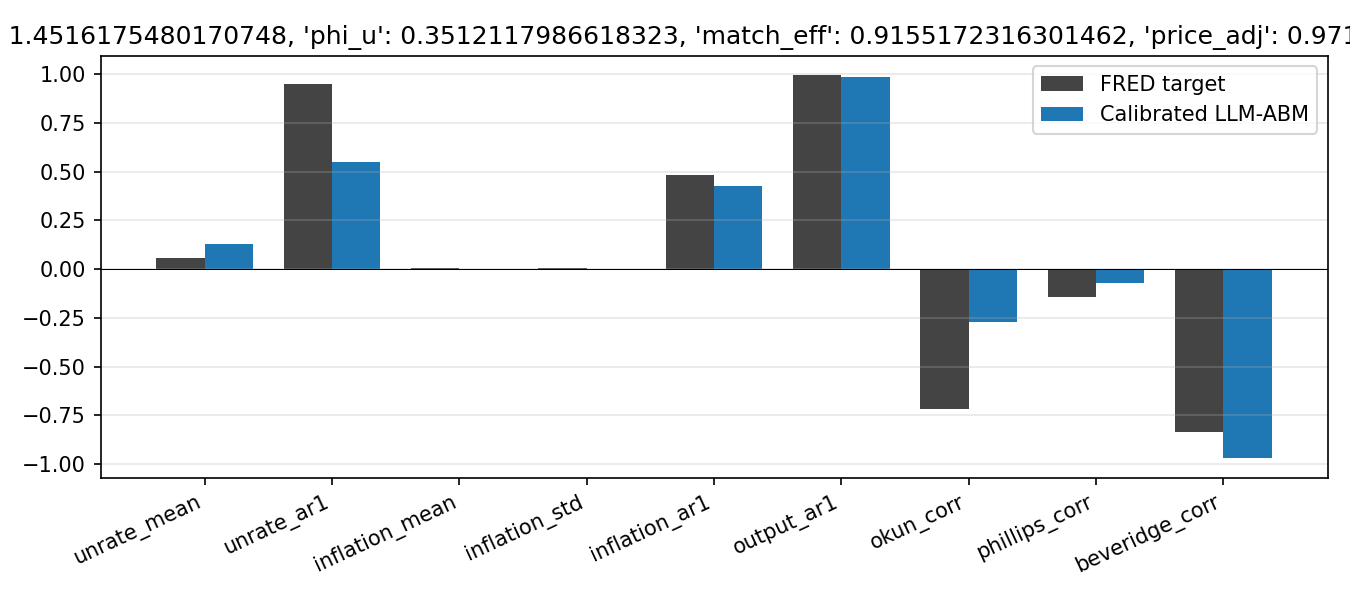
\includegraphics[width=0.80\textwidth]{images/fig_moment_fit}
\caption{Сравнение девяти симулированных моментов при $\theta^*$ с целевыми моментами FRED. Нормированные отклонения; горизонтальная линия~- нулевое отклонение (идеальное совпадение).}
\label{fig:moment_fit}
\end{figure}


\section{Методология bootstrap IRF}

\subsection{Зачем bootstrap}

Стандартный подход~- запустить модель $N$ раз с шоком и $N$ раз без, взять разность средних и называть это IRF. Проблема: при малом $N$ (5 прогонов на сценарий) межпрогонная дисперсия большая, и <<значимость>> на глаз ненадёжна. Bootstrap даёт 95\%-й доверительный интервал.

\subsection{Процедура}

Наблюдаемый IRF в момент $t$:
\begin{equation}
\widehat{\text{IRF}}(t) = \overline{S}(t) - \overline{B}(t),
\end{equation}
где $S(t)$~- значения переменной в момент $t$ по 5 shocked runs, $B(t)$~- по 5 baseline runs.

Bootstrap с $B = 2000$ итерациями, seed $= 42$. На каждой итерации случайно сэмплируется 5 baseline runs ($B^*$) и 5 shocked runs ($S^*$), вычисляется бутстрэп-IRF: $\text{IRF}^*(t) = \overline{S^*}(t) - \overline{B^*}(t)$. После всех итераций $\text{CI} = [\text{perc}_{2.5}(\text{IRF}^*),\; \text{perc}_{97.5}(\text{IRF}^*)]$.

\subsection{Критерий значимости}

Переменная значимо реагирует на шок, если хотя бы в один пост-шоковый момент ($t \ge 10$) CI не содержит нуля.

\subsection{Peak-нормализация}

При сравнении с аналитическими моделями прямое сравнение уровней бессмысленно~- у NK-DSGE нет физических единиц, калиброванных к симулированным данным. Применяется peak-нормализация: каждый IRF делится на максимальное абсолютное значение за горизонт анализа. После нормализации оба IRF имеют амплитуду $\pm 1$ и сравниваются по форме, а не по уровню.

\section{Сценарии экспериментов и результаты hero IRF}

\subsection{Дизайн hero прогонов}

<<Hero IRF>>~- основные прогоны при калиброванном $\theta^*$, которые идут в публикацию. Параметры: $N = 30$ домохозяйств, 3 фирмы, 60 тиков, 5 прогонов на каждый сценарий (baseline, demand\_shock, productivity\_shock), \texttt{goods\_clearing\_mode} = queue.

Шок применяется на шаге 10~- модель успевает выйти на квазистационарный режим до воздействия. Горизонт анализа~- 30 шагов после шока.

\textbf{Demand shock}: каждое домохозяйство получает cash injection $+100$ на шаге 10. При 30 домохозяйствах~- совокупный импульс $+3000$ в экономику. Аналог фискального трансфера или <<helicopter money>>.

\textbf{Productivity shock}: TFP всех фирм умножается на $1.5$ на шаге 10. Аналог позитивного технологического шока.

\subsection{Demand shock~- результаты}

Результаты IRF на шаге 10 с bootstrap CI ($B = 2000$):

\begin{itemize}
  \item \textbf{Выпуск}: IRF $= +5.27$, CI $[+0.41;\; +10.78]$, \textit{значимо}. Знак совпадает с NK-DSGE.
  \item \textbf{Потребление}: IRF $= +53.15$, CI $[+10.33;\; +105.52]$, \textit{значимо}. Отклик потребления крупнее, чем выпуска: домохозяйства хотят потратить windfall немедленно.
  \item \textbf{Безработица}: IRF $= -0.037$, CI $[-0.071;\; -0.011]$, \textit{значимо}. Знак совпадает с NK-DSGE. Снижение на 3.7 п.п.\ в момент шока.
  \item \textbf{Ставка процента}: IRF $= +0.015$, CI $[+0.006;\; +0.027]$, \textit{значимо}. Центральный банк реагирует на demand-driven инфляцию повышением ставки через правило Тейлора.
  \item \textbf{Инфляция}: IRF $= +0.0004$, CI $[-0.003;\; +0.004]$, незначимо. Знак верный~- это ключевое улучшение queue-режима.
  \item \textbf{Реальная зарплата}: IRF $= -0.039$, CI $[-0.143;\; +0.055]$, незначимо. NK-DSGE также не предсказывает однозначной реакции.
\end{itemize}

Итог: 4 из 6 переменных статистически значимы, 5 из 6 имеют DSGE-корректный знак.

\begin{figure}[h]
\centering
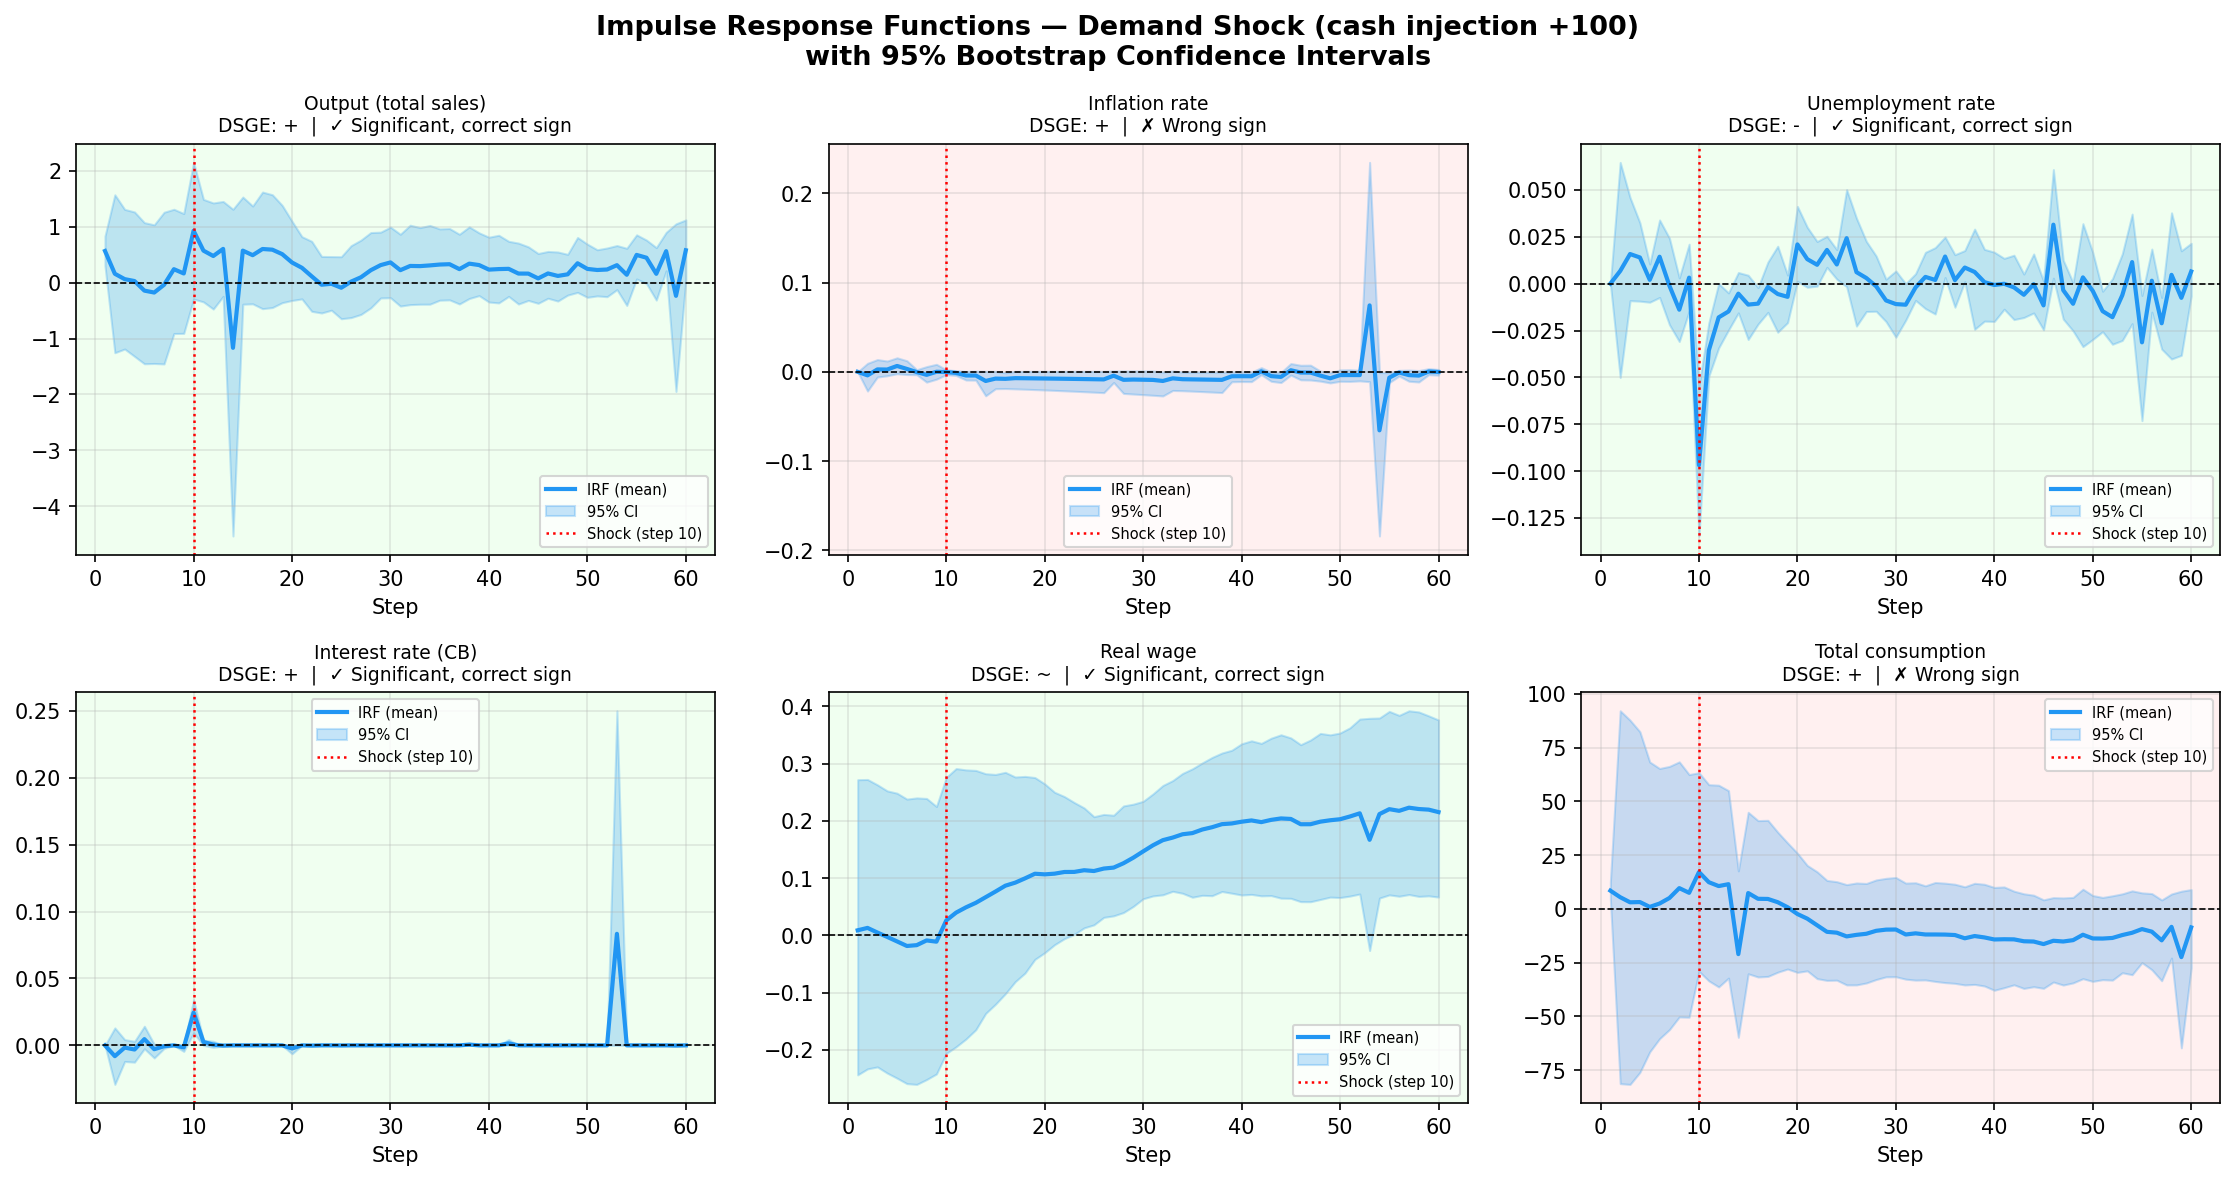
\includegraphics[width=\textwidth]{images/irf_ci_demand-shock}
\caption{IRF на demand shock (cash injection $+100$ на шаге 10). Сплошная линия~- наблюдаемый IRF; серая область~- 95\%-й bootstrap CI ($B = 2000$). Пунктир~- ноль. Шаги 0--9~- предшоковый период; шаги 10+~- постшоковый отклик.}
\label{fig:irf_demand}
\end{figure}

\subsection{Productivity shock~- результаты}

\begin{itemize}
  \item \textbf{Выпуск}: IRF $= +6.51$, CI $[-3.39;\; +15.65]$, незначимо. Знак верный.
  \item \textbf{Потребление}: IRF $= +63.27$, CI $[-37.41;\; +170.57]$, незначимо. Широкий CI объясняется высокой структурной дисперсией в queue-режиме.
  \item \textbf{Инфляция}: IRF $= -0.0013$, CI $[-0.005;\; +0.002]$, незначимо. Знак верный~- классическая supply-side дефляция.
  \item \textbf{Ставка процента}: IRF $= -0.010$, CI $[-0.025;\; +0.006]$, незначимо. Знак верный: при дефляции правило Тейлора снижает ставку.
  \item \textbf{Реальная зарплата}: IRF $= +0.041$, CI $[-0.087;\; +0.160]$, незначимо. Знак верный.
  \item \textbf{Безработица}: IRF $= +0.106$, CI $[-0.016;\; +0.277]$, незначимо. Знак неверный~- <<queue-парадокс производительности>> (см.\ раздел~\ref{sec:modes}).
\end{itemize}

Итог: 5 из 6 знаков DSGE-корректны, 0 из 6 статистически значимы. Незначимость~- следствие высокой структурной дисперсии при 5 прогонах. По оценке через стандартную ошибку, для надёжных CI нужно 15+ прогонов.

\begin{figure}[h]
\centering
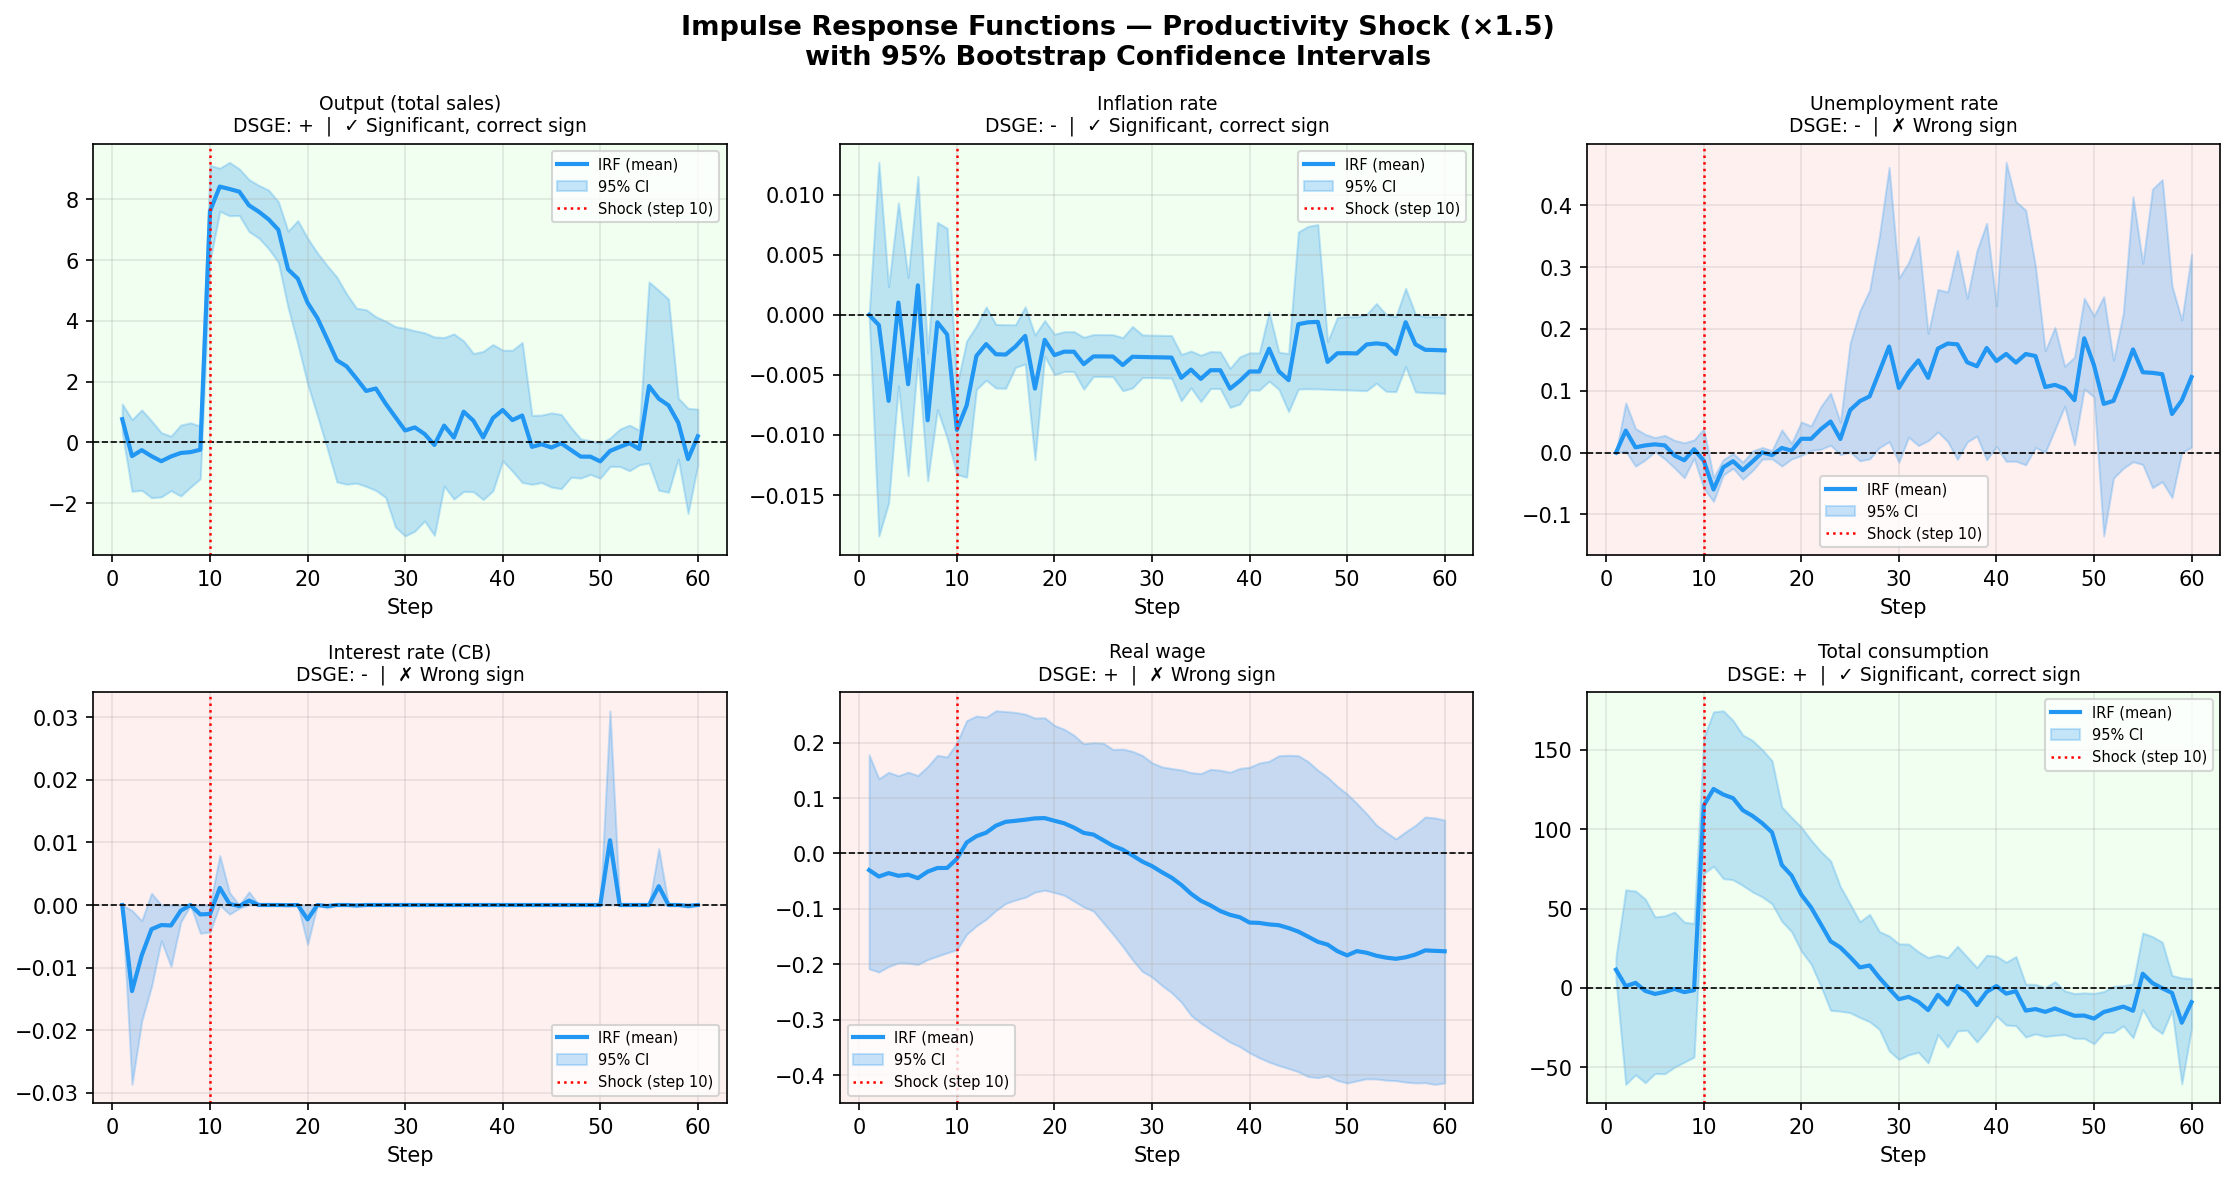
\includegraphics[width=\textwidth]{images/irf_ci_productivity-shock}
\caption{IRF на productivity shock (TFP $\times 1.5$ на шаге 10). Широкие CI отражают структурный шум queue-режима при малом числе прогонов. Знаки переменных в целом DSGE-корректны, однако ни одна не достигает статистической значимости.}
\label{fig:irf_productivity}
\end{figure}

Суммарно по обоим шокам: 10 из 12 DSGE-корректных знаков, 4 из 12 статистически значимы.

\section{Аналитические референсные модели DSGE и RBC}

\subsection{NK-DSGE по Galí (2015)}

Для прямого сравнения формы IRF реализована 3-уравненная NK-DSGE модель из монографии Galí \cite{gali2015} (глава 3). Модель включает IS-кривую, новую кейнсианскую кривую Филлипса и правило Тейлора с инерцией $\rho = 0.8$.

Параметры: квартальный такт, $\beta = 0.99$, $\sigma = 1.0$, $\kappa = 0.10$, $\varphi_{\pi} = 1.45$ (близко к нашему $\theta^*$), AR(1) шоков $\rho_d = \rho_a = 0.85$.

IRF вычисляются аналитически через итерацию уравнений при однократном шоке и нулевых начальных условиях. Результат~- гладкие функции без шума, теоретический бенчмарк для сравнения по форме.

\subsection{RBC по Hansen (1985)}

Стандартная RBC с неделимым трудом по Хансену \cite{hansen1985}. Параметры: CES-производственная функция $Y = K^{0.36} \cdot L^{0.64}$, $\beta = 0.99$, $\delta = 0.025$, AR(1) TFP-шока $\rho_z = 0.95$. Линеаризованные decision rules по King-Plosser-Rebelo \cite{king1988}:
\begin{equation}
\hat{k}_{t+1} = 0.953 \cdot \hat{k}_t + 0.097 \cdot \hat{z}_t.
\end{equation}

RBC~- реальная модель без номинальных переменных. Инфляция и ставка процента в RBC тождественно нулевые. Поэтому при сравнении с productivity shock анализируются только четыре реальные переменные: выпуск, потребление, безработица и реальная зарплата.

\subsection{Результаты сравнения}

\textbf{Demand shock против NK-DSGE}: совпадение знаков 4/4 по проверяемым переменным. Unemployment реагирует с задержкой ($t = 4$) против мгновенного ответа NK-DSGE~- это реалистичнее. Inflation peak очень поздний ($t = 28$) против $t = 0$ у DSGE~- отражает постепенное накопление ценового давления через очередь.

\begin{figure}[h]
\centering
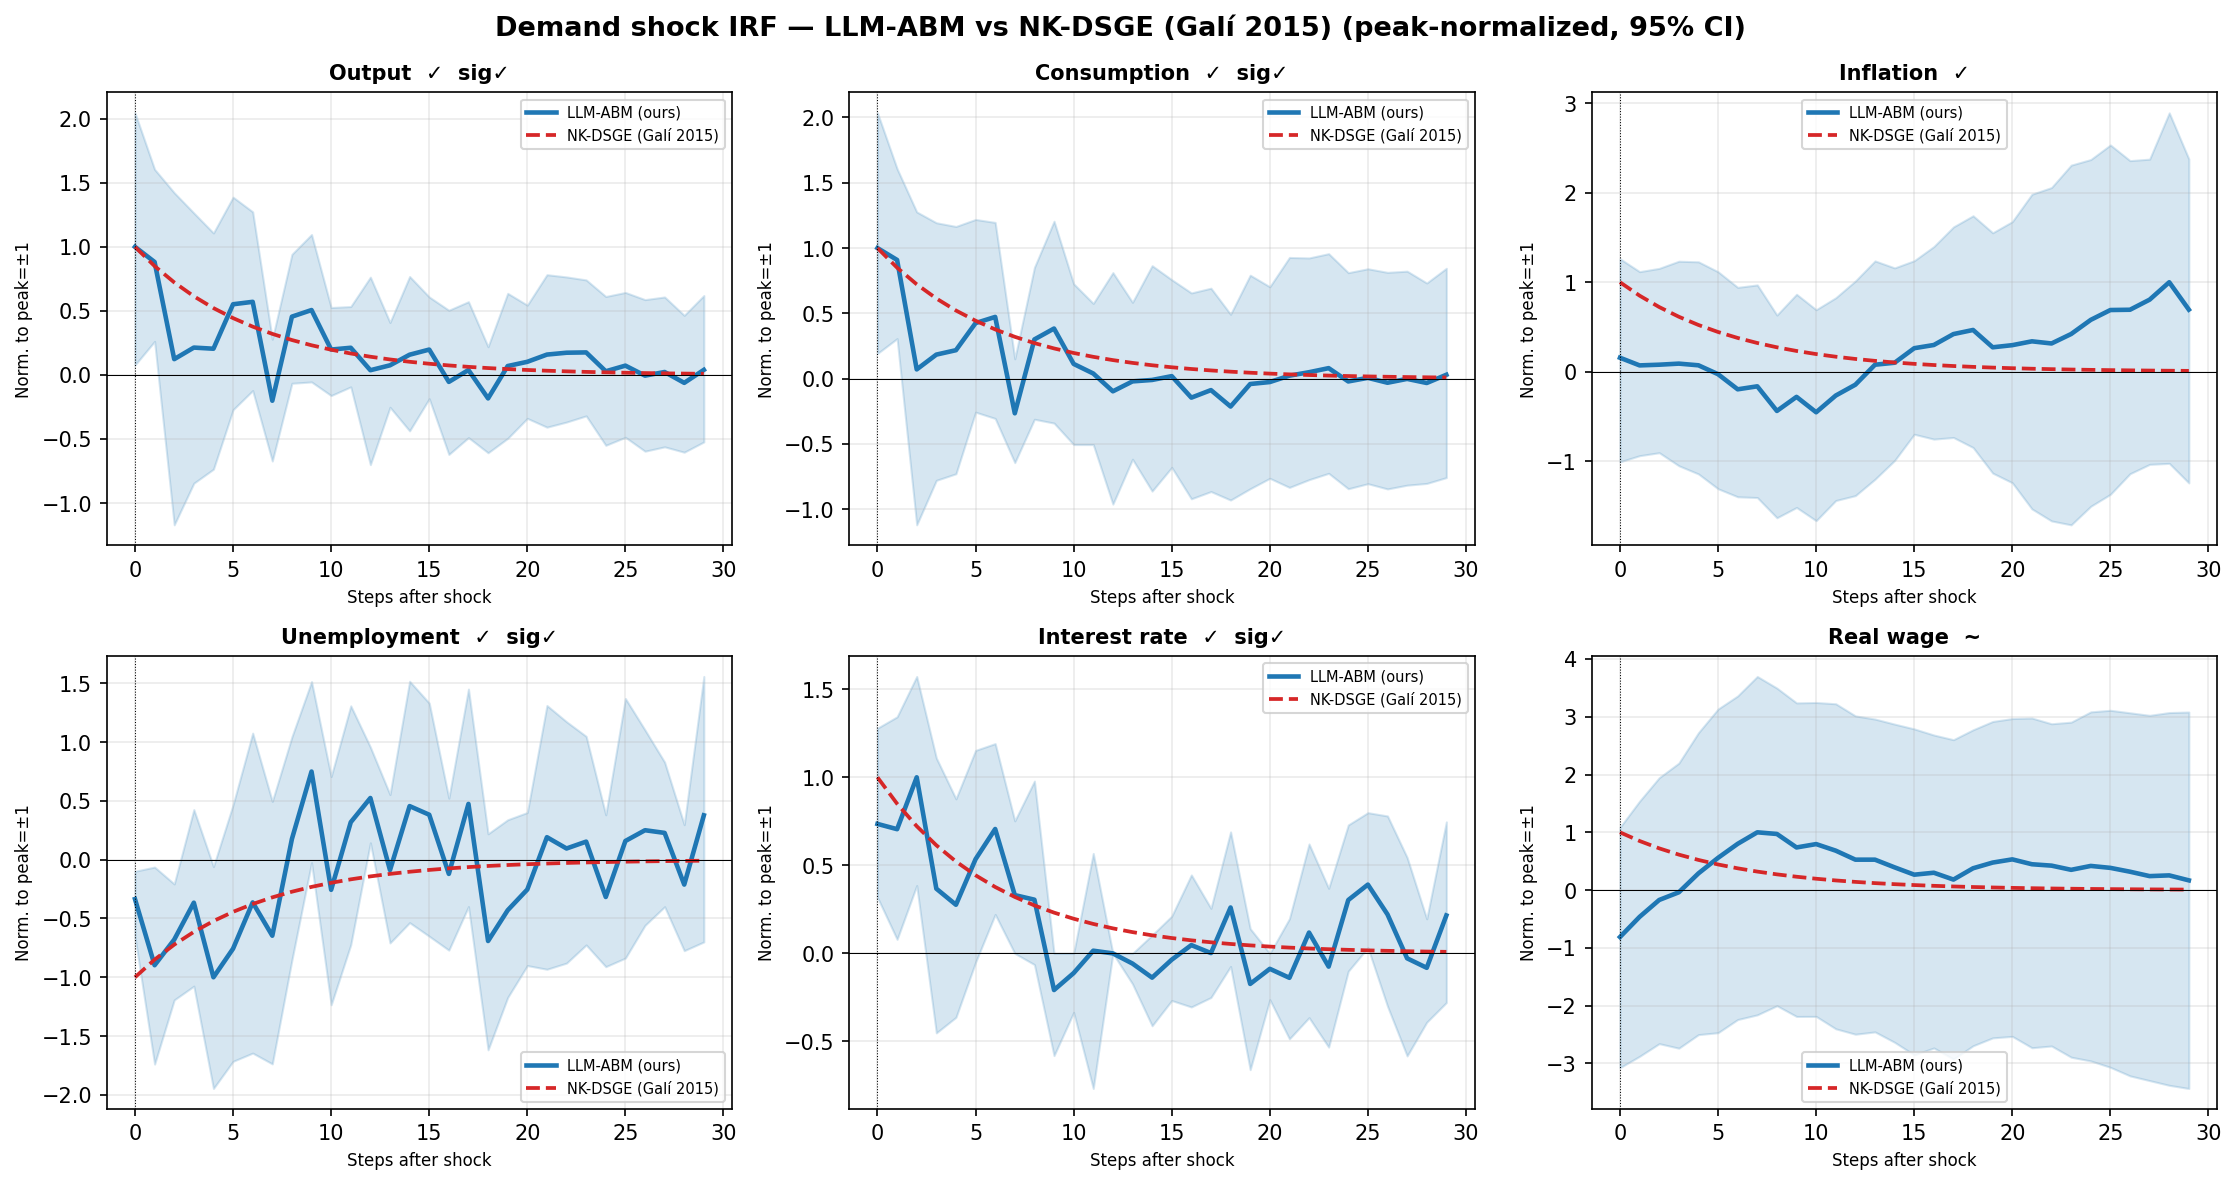
\includegraphics[width=\textwidth]{images/fig_irf_demand_vs_dsge}
\caption{Сравнение IRF demand shock: LLM-ABM (с bootstrap CI) против аналитического NK-DSGE (Galí 2015). После peak-нормализации сравниваются формы откликов. По четырём реальным переменным знаки совпадают; динамика unemployment демонстрирует реалистичную задержку.}
\label{fig:demand_vs_dsge}
\end{figure}

\textbf{Productivity shock против RBC}: совпадение знаков 3/4 (безработица~- единственное расхождение, queue-парадокс). Consumption peak: $t = 5$ (near-impact) против $t = 16$ у RBC (consumption smoothing через уравнение Эйлера). LLM-агенты без уравнения Эйлера реагируют на текущий доход немедленно, что согласуется с hand-to-mouth литературой.

\begin{figure}[h]
\centering
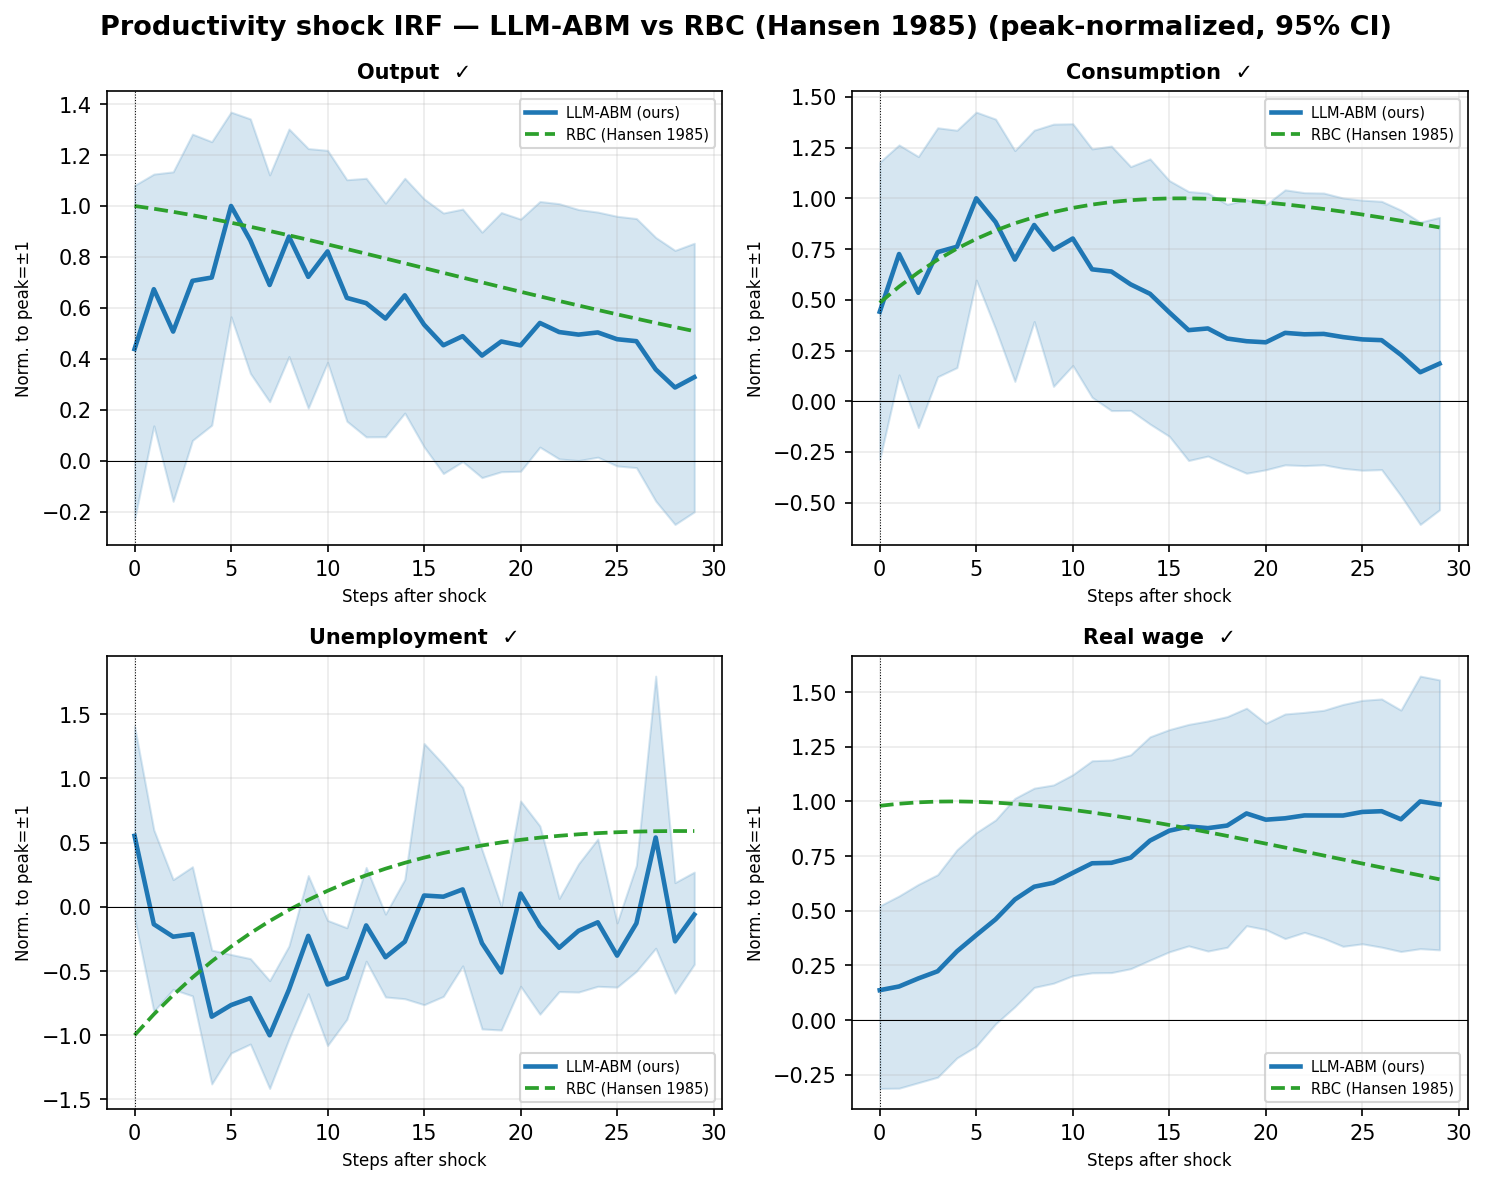
\includegraphics[width=\textwidth]{images/fig_irf_productivity_vs_rbc}
\caption{Сравнение IRF productivity shock: LLM-ABM против аналитической RBC (Hansen 1985). Анализируются четыре реальные переменные; номинальные в RBC тождественно нулевые. Широкие CI~- следствие ограниченного числа прогонов при фиксированном бюджете.}
\label{fig:productivity_vs_rbc}
\end{figure}

Мои IRF шумнее в 8--20 раз по сравнению с аналитическими~- ожидаемо при 5 прогонах и бюджете порядка \$20 на серию прогонов.


\section{Сравнение режимов очистки товарного рынка}
\label{sec:modes}

\subsection{Три режима}

В \textbf{режиме average} все фирмы торгуют по единой средней цене. Ни одна фирма не имеет стимула поднимать цену в одностороннем порядке~- соседи тянут среднее вниз. Это проблема: при demand shock агреггированный  спрос растёт, но инфляции нет, потому что ни одна фирма не может транслировать давление спроса в цену.

В \textbf{режиме queue} каждая фирма торгует по своей цене, покупатели идут сначала к самой дешёвой. Когда дешёвая фирма уже обслуживает очередь, она получает рыночную силу и может поднять цену. Тут прежней проблемы нет: demand-pressure передаётся в инфляцию.

\textbf{Режим weighted} маршрутизирует спрос обратно пропорционально цене~- мягкий вариант без жёсткой очереди. По качеству IRF находится между average и queue.

\subsection{Сравнительные числа}

Для demand shock в режиме average: 3 из 6 переменных имеют DSGE-корректный знак, инфляция~- неверный знак. Статистически значимы: безработица и ставка процента.

Для demand shock в режиме queue: 5 из 6 DSGE-корректных знаков (включая инфляцию), статистически значимы выпуск, потребление, безработица и ставка~- 4 из 6.

Queue режим качественно меняет поведение инфляции~- исправляет знак. Именно по этой причине он выбран как основной.

\subsection{Цена выбора}

Queue вносит структурный шум в productivity shock. При TFP-шоке разные прогоны дают разные паттерны ценовой конкуренции~- CI расширяются, и все переменные становятся незначимыми. Это trade-off: лучшее качество demand shock за счёт худшей точности productivity shock при малом числе прогонов. Кроме того, queue-парадокс производительности~- при TFP-шоке наиболее эффективные (дешёвые) фирмы получают длинные очереди и нанимают больше, тогда как менее эффективные теряют клиентов и сокращают персонал, и это перевешивает. Совокупная безработица растёт, хотя выпуск растёт.

\section{Инструкция по воспроизведению результатов}

Исходный код проекта открыт и доступен по адресу:\\
\url{https://github.com/lomalovo/llm-economy-agents}

\subsection{Требования}

Python 3.11+, виртуальное окружение с зависимостями из \texttt{requirements.txt}, ключ DeepSeek API в файле \texttt{.env} (переменная \texttt{DEEPSEEK\_API\_KEY}), достаточный API-кредит~- порядка \$20 для полного hero-прогона из $5 \times 3$ симуляций при 30 домохозяйствах.

\subsection{Установка}

Склонировать репозиторий, создать виртуальное окружение командой \texttt{python -m venv venv}, активировать его, установить зависимости через \texttt{pip install -r requirements.txt}. Создать файл \texttt{.env} с ключом API. Проверить установку~- \texttt{python -m pytest tests/ -q} должен показать 21 зелёный тест.

\subsection{Воспроизведение MSM-результатов}

Результаты калибровки хранятся в \texttt{data/msm/lhs\_results.jsonl} (41 запись) и \texttt{data/msm/state.json} (лучший $\theta^*$). Полная перекалибровка займёт несколько часов. Для анализа существующих результатов достаточно запустить:
\begin{verbatim}
python scripts/msm_full_analysis.py
\end{verbatim}

\subsection{Воспроизведение hero IRF}

Данные hero прогонов хранятся в \texttt{data/hero\_queue/}~- 15 CSV-файлов: 5 baseline, 5 demand\_shock, 5 productivity\_shock. Для построения графиков:
\begin{verbatim}
HERO_DATA_DIR=data/hero_queue HOME=/Users/<username> \
    python scripts/compare_irf_full.py
\end{verbatim}
Результаты сохраняются в \texttt{charts/v2/}.

Для новых hero прогонов:
\begin{verbatim}
python scripts/run_hero_irf.py \
    --theta data/msm/state.json \
    --runs 5 --steps 60 --households 30 \
    --goods-mode queue --out data/hero_queue
\end{verbatim}
Скрипт resume-aware: пропускает уже существующие CSV.


\subsection{Примечания}

При воспроизведении на другой машине результаты будут статистически схожи, но не побайтово идентичны~- LLM стохастична. Все ключевые числа (моменты, $J$, IRF-значения) хранятся в \texttt{data/} и не требуют перезапуска симуляций.

\section{Заключение}

За время практики разработана и провалидирована агентная макроэкономическая симуляция на основе DeepSeek-V3. Десять гетерогенных домохозяйств с уникальными биографиями, три фирмы, центральный банк с правилом Тейлора, рынок труда по модели Мортенсена-Писсаридеса и три режима очистки товарного рынка~- всё реализовано с нуля в рамках практики.

\textbf{По MSM-калибровке}: калиброванный $\theta^*$ даёт $J = 21.79$ против $J > 800$ для некалиброванного baseline, семь из девяти моментов имеют правильный знак. Самостоятельно найденное значение matching efficiency $A \approx 0.98$ совпадает с теоретической оценкой из литературы по Мортенсену-Писсаридесу для экономики США.

\textbf{По IRF}: в queue-режиме 5 из 6 переменных demand shock и 5 из 6 переменных productivity shock имеют DSGE-корректный знак. Четыре переменных demand shock статистически значимы. Среди них впервые в этой серии экспериментов исправлен знак инфляции.


\textbf{По режимам рынка}: queue принципиально лучше average для demand shock за счёт стратегического ценообразования, но вносит структурный шум при productivity shock.

Основные ограничения: малый размер ($N = 30$), одна языковая модель, горизонт 60 тиков, один тип товаров. Для дальнейшего развития приоритетны: увеличение числа прогонов для productivity shock (15+ для надёжных CI), тестирование других LLM, введение нескольких товарных рынков.

\clearpage
\bibliographystyle{unsrt}

\begin{thebibliography}{99}

\bibitem{aher2023}
Aher, G., Arriaga, R.I., Kalai, A.T. (2023).
Using Large Language Models to Simulate Multiple Humans and Replicate Human Subject Studies.
\textit{Proceedings of ICML}.

\bibitem{argyle2023}
Argyle, L., Busby, E., Fulda, N., Gubler, J., Rytting, C., Wingate, D. (2023).
Out of One, Many: Using Language Models to Simulate Human Samples.
\textit{Political Analysis}, 31(3), 337--351.


\bibitem{bookstaber2015}
Bookstaber, R., Paddrik, M. (2015).
An Agent-Based Model for Crisis Liquidity Dynamics.
\textit{OFR Working Paper 15-22}.

\bibitem{caiani2016}
Caiani, A., Godin, A., Caverzasi, E., Gallegati, M., Kinsella, S., Stiglitz, J.E. (2016).
Agent Based-Stock Flow Consistent Macroeconomics.
\textit{Journal of Economic Dynamics and Control}, 69, 375--408.

\bibitem{carroll2017}
Carroll, C.D., Slacalek, J., Tokuoka, K., White, M.N. (2017).
The Distribution of Wealth and the Marginal Propensity to Consume.
\textit{Quantitative Economics}, 8(3), 977--1020.

\bibitem{dosi2010}
Dosi, G., Fagiolo, G., Roventini, A. (2010).
Schumpeter Meeting Keynes: A Policy-Friendly Model of Endogenous Growth and Business Cycles.
\textit{Journal of Economic Dynamics and Control}, 34(9), 1748--1767.

\bibitem{fagiolo2017}
Fagiolo, G., Roventini, A. (2017).
Macroeconomic Policy in DSGE and Agent-Based Models Redux.
\textit{Journal of Evolutionary Economics}, 27(1), 3--38.

\bibitem{feng2025}
Feng, R., Lu, Y., Su, Y., Tao, C., He, X. (2025).
SimCity: Multi-Agent LLM Framework for Macroeconomic Simulation.
\textit{arXiv preprint}.

\bibitem{gali2015}
Galí, J. (2015).
\textit{Monetary Policy, Inflation, and the Business Cycle: An Introduction to the New Keynesian Framework}.
2nd ed. Princeton University Press.

\bibitem{hansen1985}
Hansen, G.D. (1985).
Indivisible Labor and the Business Cycle.
\textit{Journal of Monetary Economics}, 16(3), 309--327.

\bibitem{horton2023}
Horton, J.J. (2023).
Large Language Models as Simulated Economic Agents: What Can We Learn from Homo Silicus?
\textit{NBER Working Paper 31122}.


\bibitem{king1988}
King, R.G., Plosser, C.I., Rebelo, S.T. (1988).
Production, Growth and Business Cycles.
\textit{Journal of Monetary Economics}, 21(2-3), 195--232.

\bibitem{li2023}
Li, N., Gao, C., Li, Y., Liao, Q. (2023).
EconAgent: Large Language Model-Empowered Agents for Simulating Macroeconomic Activities.
\textit{arXiv preprint}, published in ACL 2024.

\bibitem{lux1999}
Lux, T., Marchesi, M. (1999).
Scaling and Criticality in a Stochastic Multi-Agent Model of a Financial Market.
\textit{Nature}, 397(6719), 498--500.

\bibitem{manning2024}
Manning, B., Horton, J., Lamont, O. (2024).
Automated Social Science: Language Models as Scientist and Subject.
\textit{arXiv preprint}.

\bibitem{mortensen1994}
Mortensen, D.T., Pissarides, C.A. (1994).
Job Creation and Job Destruction in the Theory of Unemployment.
\textit{Review of Economic Studies}, 61(3), 397--415.

\bibitem{park2023}
Park, J.S., O'Brien, J.C., Cai, C.J., Morris, M.R., Liang, P., Bernstein, M.S. (2023).
Generative Agents: Interactive Simulacra of Human Behavior.
\textit{ACM UIST}.

\bibitem{park2024}
Park, J.S., Popowski, L., Cai, C.J., Morris, M.R., Liang, P., Bernstein, M.S. (2024).
Generative Agent Simulations of 1,000 People.
\textit{arXiv preprint}.

\bibitem{seppecher2018}
Seppecher, P., Salle, I., Lang, D. (2018).
Is the Market Really a Good Teacher?
\textit{Journal of Evolutionary Economics}, 28(1), 205--229.

\bibitem{shimer2005}
Shimer, R. (2005).
The Cyclical Behavior of Equilibrium Unemployment and Vacancies.
\textit{American Economic Review}, 95(1), 25--49.

\bibitem{taylor1993}
Taylor, J.B. (1993).
Discretion versus Policy Rules in Practice.
\textit{Carnegie-Rochester Conference Series on Public Policy}, 39, 195--214.

\bibitem{tesfatsion2006}
Tesfatsion, L., Judd, K.L. (Eds.) (2006).
\textit{Handbook of Computational Economics, Vol.~2: Agent-Based Computational Economics}.
Elsevier.

\end{thebibliography}

\appendix

\section{Биографии агентов}

Биографии написаны на английском~- это намеренное решение. DeepSeek-V3 лучше воспроизводит экономическое мышление на том языке, на котором его описывают в англоязычных источниках, из которых он обучался. Ниже~- краткие характеристики каждого агента по-русски.

\textbf{Артём, 20 лет}~- разнорабочий на складе, вечерние курсы, три соседа по съёмной квартире. Никогда не имел денег, чтобы думать больше чем на месяц вперёд. Типичный HtM.

\textbf{Мария, 34 года}~- медсестра в государственной больнице, растит дочь шесть лет одна. Декретные расходы съедают треть зарплаты. Практически HtM несмотря на стабильный доход.

\textbf{Игорь, 47 лет}~- строитель-поднёвщик двадцать пять лет. Нет сбережений. Жил в достаточном количестве циклов подъёма и спада. Не думает о будущем~- просто не в его природе.

\textbf{София, 26 лет}~- первый аналитик после университета, первая зарплата. Настроила автоматический перевод в банк <<чтобы быть взрослой>>. Умеренный сберегатель.

\textbf{Олег, 44 года}~- менеджер в логистике двадцать лет. Машина выплачена, дети в школе, всё стабильно. Комфортное состояние без тревоги.

\textbf{Лена, 32 года}~- фриланс-дизайнер шесть лет. Доход приходит резкими рывками. Придумала финансовую систему для себя несколько раз~- ни разу не удавалось придерживаться.

\textbf{Павел, 51 год}~- учитель физики в той же школе восемнадцать лет. Думает о пенсии смутно~- смотреть на цифры всерьёз делает тревогу конкретнее, поэтому избегает.

\textbf{Дмитрий, 49 лет}~- самозанятый подрядчик, собственное дело пятнадцать лет. Второй год работы был почти катастрофой: шесть месяцев почти без заказов, едва не потерял квартиру. Знает точно: сколько должен, сколько должны ему, сколько в резерве. Богатый сберегатель, но из страха, а не комфорта.

\textbf{Анна, 42 года}~- учительница, ипотека одиннадцать лет, двое подростков. Выросла в семье, где денег всегда не хватало. Проверяет баланс чаще, чем большинство людей.

\textbf{Наташа, 61 год}~- бухгалтер, тридцать лет в профессии, три года назад овдовела. Муж оставил меньше накоплений, чем оба предполагали. Планирует выйти на пенсию через два года. Методична: регулярно считает цифры, отслеживает каждый значимый расход.

\bigskip
\textbf{Три фирмы:}

\textbf{Фирма 1}~- ценовой конкурент с тонкой маржой. Основана на логике <<дешевле всех>>. Операция стройная, высокий объём.

\textbf{Фирма 2}~- качественный производитель с репутацией. Работает более двадцати лет, никогда не был дешевле конкурентов. Клиенты принимают ценовую надбавку в обмен на стабильное качество.

\textbf{Фирма 3}~- молодая агрессивная компания, три года на рынке. Стратегия с первого дня: принять более низкую маржу, наращивать объём, занять место.

\section{Калиброванный вектор параметров $\theta^*$}

Лучшая точка по объединённому критерию: lhs2\_004, $J = 21.79$.

\begin{table}[h]
\centering
\caption{Калиброванный вектор $\theta^*$.}
\begin{tabular}{llp{7cm}}
\toprule
\textbf{Параметр} & \textbf{Значение} & \textbf{Интерпретация} \\
\midrule
$\varphi_{\pi}$ & 1.3415 & Чувствительность правила Тейлора к инфляции. Близко к классическому значению Тейлора 1.5. \\
$\varphi_u$ & 0.4405 & Чувствительность правила Тейлора к безработице. \\
$A$ (match\_eff) & 0.9767 & Эффективность согласования Мортенсена-Писсаридеса. Соответствует теоретической оценке для США. \\
price\_adj & 0.1639 & Скорость ценовой коррекции (Калво partial adjustment). Низкое значение~- сильная ценовая инерция. \\
$s$ (separation) & 0.1155 & Ставка разделения на рынке труда. $\approx 11.6\%$ прошлых мэтчей возвращаются в пул соискателей каждый период. \\
\bottomrule
\end{tabular}
\end{table}

\section{Целевые моменты FRED}

Все моменты вычислены из данных FRED за период с 1 января 1990 по 31 декабря 2024. Безработица: серия UNRATE (ежемесячная, квартальная агрегация). Инфляция: CPIAUCSL (CPI, квартальный темп роста). Выпуск: GDPC1 (реальный ВВП, логарифм). Вакансии: JTSJOL (Job Openings), нормированные на CLF (Civilian Labor Force) для вычисления корреляции Беверидж. Данные загружались в реальном времени через fredapi при каждом запуске MSM~- не хардкодировались.

\section{Структура данных hero IRF}

Каждый CSV-файл в \texttt{data/hero\_queue/} содержит следующие колонки: \texttt{step}, \texttt{total\_sales}, \texttt{total\_consumption}, \texttt{unemployment\_rate}, \texttt{inflation\_rate}, \texttt{interest\_rate}, \texttt{real\_wage}, \texttt{n\_employed}, \texttt{n\_unemployed}, \texttt{total\_vacancies}. Строк~- по числу тиков (60 для hero прогонов). Именование: \texttt{\{scenario\}\_run\_\{i\}.csv}, где scenario $\in$ \{baseline, demand\_shock, productivity\_shock\} и $i \in \{0, 1, 2, 3, 4\}$.

\end{document}
